\documentclass{beamer}


\makeatletter
\newcommand*\Alt{\alt{\Alt@branch0}{\Alt@branch1}}

\newcommand\Alt@branch[3]{%
  \begingroup
  \ifbool{mmode}{%
    \mathchoice{%
      \Alt@math#1{\displaystyle}{#2}{#3}%
    }{%
      \Alt@math#1{\textstyle}{#2}{#3}%
    }{%
      \Alt@math#1{\scriptstyle}{#2}{#3}%
    }{%
      \Alt@math#1{\scriptscriptstyle}{#2}{#3}%
    }%
  }{%
    \sbox0{#2}%
    \sbox1{#3}%
    \Alt@typeset#1%
  }%
  \endgroup
}

\newcommand\Alt@math[4]{%
  \sbox0{$#2{#3}\m@th$}%
  \sbox1{$#2{#4}\m@th$}%
  \Alt@typeset#1%
}

\newcommand\Alt@typeset[1]{%
  \ifnumcomp{\wd0}{>}{\wd1}{%
    \def\setwider   ##1##2{##2##1##2 0}%
    \def\setnarrower##1##2{##2##1##2 1}%
  }{%
    \def\setwider   ##1##2{##2##1##2 1}%
    \def\setnarrower##1##2{##2##1##2 0}%
  }%
  \sbox2{}%
  \sbox3{}%
  \setwider2{\wd}%
  \setwider2{\ht}%
  \setwider2{\dp}%
  \setnarrower3{\ht}%
  \setnarrower3{\dp}%
  \leavevmode
  \rlap{\usebox#1}%
  \usebox2%
  \usebox3%
}
\makeatother

\usetheme[block=fill]{metropolis}




\usepackage[utf8]{inputenc}
\usepackage[T1]{fontenc}
\usepackage[english]{babel}

\usepackage{amsmath}
\usepackage{tikz}
\usepackage{mathrsfs}



\newcommand{\R}{\ensuremath{\mathbb{R}}}
\newcommand{\Rb}{\ensuremath{\overline{\mathbb{R}}}}
\newcommand{\N}{\ensuremath{\mathbb{N}}}
\newcommand{\Q}{\ensuremath{\mathbb{Q}}}
\newcommand{\Z}{\ensuremath{\mathbb{Z}}}
\newcommand{\C}{\ensuremath{\mathbb{C}}}
\newcommand{\U}{\ensuremath{\mathbb{U}}}
\newcommand{\F}{\ensuremath{\mathbb{F}}}
\newcommand{\K}{\ensuremath{\mathbb{K}}}
\newcommand{\TODO}{\textbf{TODO}}


\newcommand\eqdef{\stackrel{\mathclap{\mbox{\tiny def}}}{=}}


\newcommand{\ket}[1]{|#1\rangle}
\newcommand{\bra}[1]{\langle#1|}
\newcommand{\braket}[2]{\langle#1|#2\rangle}

\newcommand{\dd}{\mathrm{d}}
\newcommand{\der}[2]{\frac{\dd{#1}}{\dd{#2}}}
\newcommand{\dern}[3]{\frac{\dd^{#3} #1}{\dd{#2}^{#3}}}
\newcommand{\dpar}[2]{\frac{\partial{#1}}{\partial{#2}}}
\newcommand{\dparn}[3]{\frac{\partial^{#3} {#1}}{\partial{#2}^{#3}}}


\newcommand{\mat}[1]{\begin{pmatrix}#1\end{pmatrix}}
\newcommand{\bs}{\boldsymbol}

\newcommand{\Tr}{\mathsf{Tr}\,}
\newcommand{\argmax}{\mathop{\mathsf{arg\,max}}}
\newcommand{\argmin}{\mathop{\mathsf{arg\,min}}}
\newcommand{\rk}{\mathsf{rk}\,}
\newcommand{\Span}{\mathsf{Span}\,}
\newcommand{\diag}{\mathsf{diag}\,}


\newcommand{\class}[1]{{\mathscr{C}^{#1}}}

\newcommand{\trnorm}[1]{\frac{#1}{\Tr\left({#1}\right)}}
\newcommand{\ml}{_{M\!L}}


\newcommand{\maxim}[3]{\begin{cases}
    \mathbf{maximize}\,\quad #1& \mathbf{on}\; #2\\
    \mathbf{subject\;to}\quad #3
  \end{cases}}
\newcommand{\maximf}[2]{\begin{cases}
    \mathbf{maximize}\,\quad #1& \mathbf{on}\; #2
  \end{cases}}
\newcommand{\maxima}[3]{\begin{cases}
    \mathbf{maximize}\,\quad #1& \mathbf{on}\; #2\\
    \mathbf{subject\;to}\quad \begin{aligned}[t]#3\end{aligned}
  \end{cases}}

\newcommand{\minim}[3]{\begin{cases}
    \mathbf{minimize}\;\,\quad #1& \mathbf{on}\; #2\\
    \mathbf{subject\;to}\quad #3
  \end{cases}}
\newcommand{\minimf}[2]{\begin{cases}
    \mathbf{minimize}\,\quad #1& \mathbf{on}\; #2
  \end{cases}}
\newcommand{\minima}[3]{\begin{cases}
    \mathbf{minimize}\;\,\quad #1& \mathbf{on}\; #2\\
    \mathbf{subject\;to}\quad \begin{aligned}[t]#3\end{aligned}
  \end{cases}}

\newcommand{\gap}{\hspace{0.8cm}}
\newcommand{\twoline}{\vphantom{\frac\int\int}}
\graphicspath{{../img/}}




\title{Error estimation in maximum likelihood reconstruction for
    quantum state tomography}
\author{Thibaut Pérami}
\institute{LKB, Collège de France}
\date{September 11, 2019}

\begin{document}

\maketitle

\begin{frame}{Quantum state tomography}
  \centering
    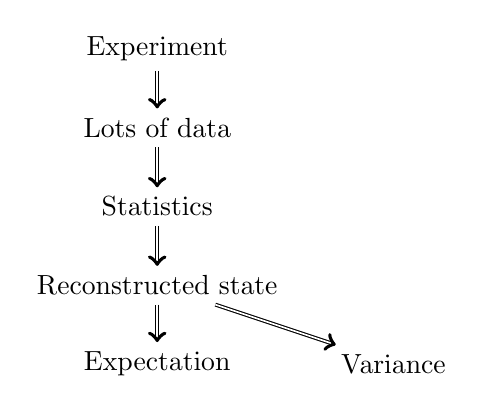
\begin{tikzpicture}
    \node[rectangle] (E) at(0,0) {Experiment};
    \pause
    \node[rectangle] (D) at(0,-1) {Lots of data};
    \draw[double,->] (E) -- (D);
    \pause
    \node[rectangle] (S) at (0,-2) {Statistics};
    \draw[double,->] (D) -- (S);
    \pause
    \node[rectangle] (R) at (0,-3) {Reconstructed state};
    \draw[double,->] (S) -- (R);
    \pause
    \node[rectangle] (Ex) at (0,-4) {Expectation};
    \draw[double,->] (R) -- (Ex);
    \pause
    \node[rectangle] (V) at (3,-4) {Variance};
    \draw[double,->] (R) -- (V);
  \end{tikzpicture}

  
\end{frame}

\section{Setup and Goal}


\begin{frame}{The experimental setup}

  \vfill

  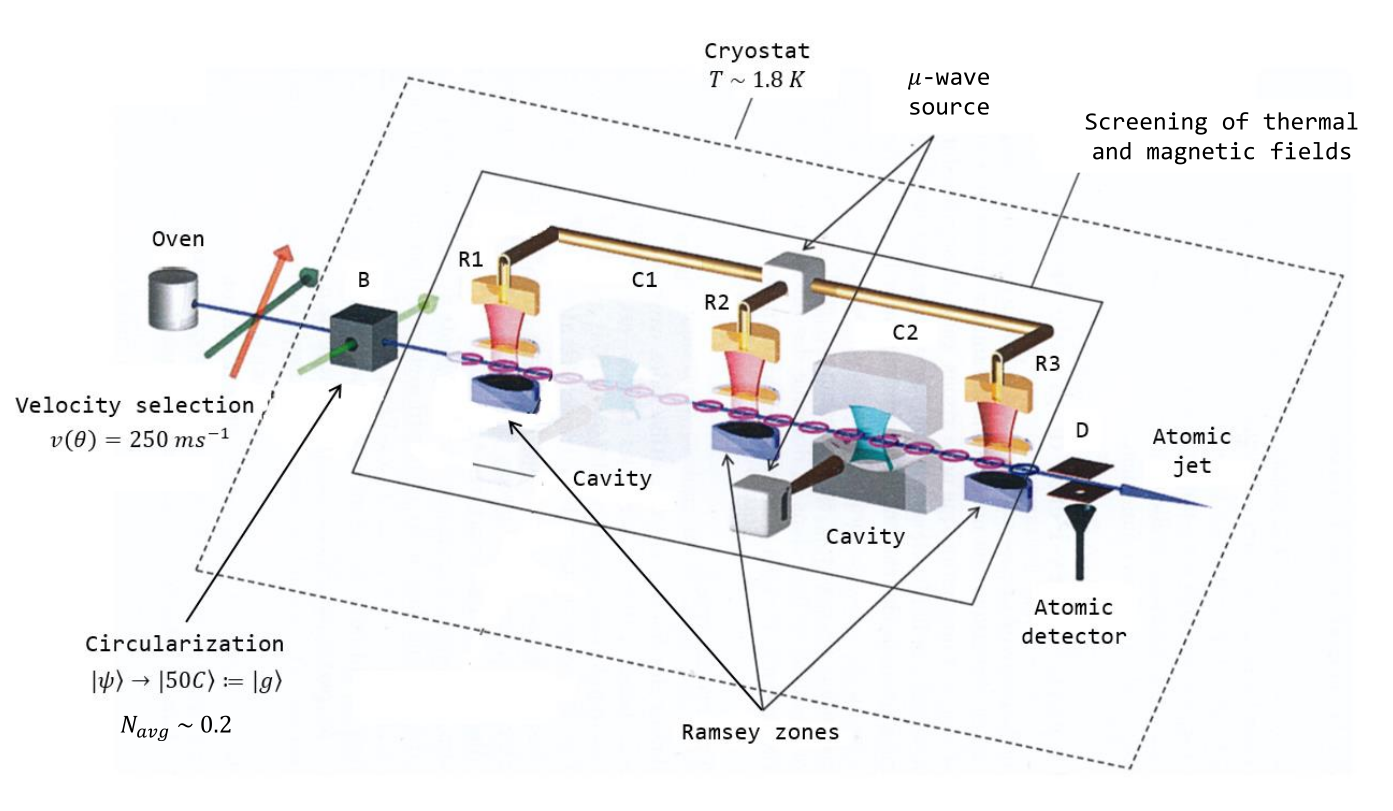
\includegraphics[width=\textwidth]{exp.png}
\end{frame}

\begin{frame}{The goal$\colon{}$ Create a Maxwell demon}

\vspace{2cm}

  \begin{description}
    \item[Normal interaction:] A cold atom \alert{takes} heat from a hot cavity
      \pause{}
    \item[Maxwell demon] A cold atom \alert{gives} heat to a hot cavity
  \end{description}

  \begin{center}
    \includegraphics[height=3cm]{md.png}
  \end{center}


\end{frame}

\section{Atoms and light in cavities}

\begin{frame}{Circular Rydberg atoms}
\begin{center}
  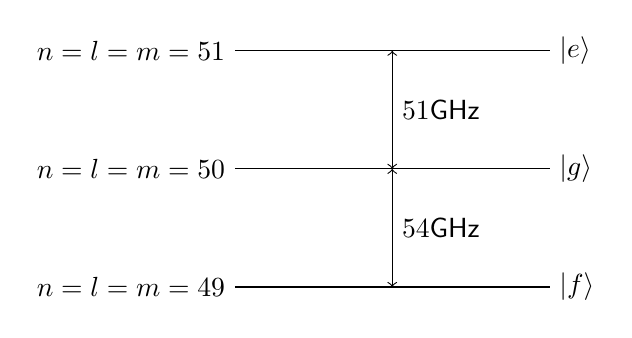
\begin{tikzpicture}[y=1.5cm,x=2cm]
    \draw (0,0) -- (2,0);
    \node[right] at (2,0) {$\ket e$};
    \node[left] at (0,0) {$n=l=m=51$};
    \draw (0,-1) -- (2,-1);
    \node[right] at (2,-1) {$\ket g$};
    \node[left] at (0,-1) {$n=l=m=50$};
    \draw[<->] (1,0) --(1,-1);
    \node[right] at (1,-0.5) {$ 51 \mathsf{GHz}$};
    \pause{}
    \draw (0,-2) -- (2,-2);
    \node[right] at (2,-2) {$\ket f$};
    \node[left] at (0,-2) {$n=l=m=49$};
    \draw[<->] (1,-1) --(1,-2);
    \node[right] at (1,-1.5) {$54 \mathsf{GHz}$};


  \end{tikzpicture}
\end{center}

\vfill

  \begin{block}<3->{Hamiltonian on a transition}
    \[H = \frac{\hbar \omega}2 \sigma_Z\]
  \end{block}

\end{frame}

\begin{frame}{Rydberg atoms in a classical field: Rabi oscillation}
  \[H = \frac{\hbar \omega}2 \sigma_Z \pause - \bs D \cdot \bs E\]

  \pause{}

  \begin{block}{Secular approximation in interaction picture: Rabi oscillation}
    \[H_1 = \frac{\hbar \Delta_r}2 \sigma_Z - \frac{\hbar \Omega_r}2
      \mat{0&e^{i\phi}\\e^{-i\phi}&0} = \frac{\hbar \Omega_r'}2 \bs \sigma
      \cdot \bs n\]
  \end{block}

  \pause{}

  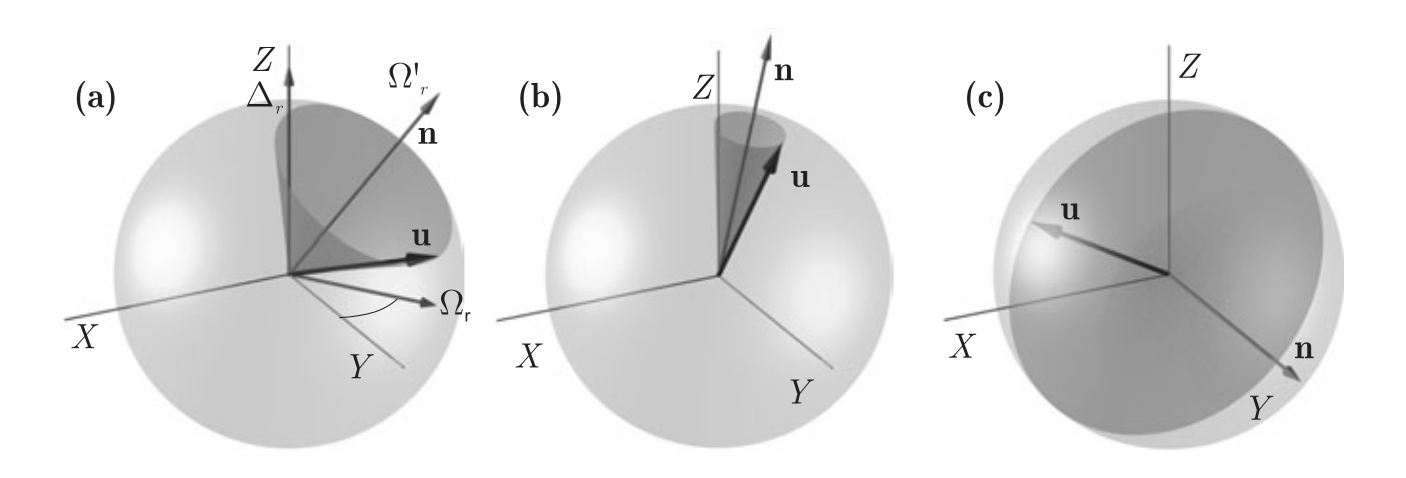
\includegraphics[width=\textwidth]{Rabi.png}
\end{frame}

\begin{frame}{EM field in a resonant cavity}
  \[H = \hbar\omega \left(N +\frac12\right)\]

  \[a = \sum_n \sqrt{n} \ket {n-1} \bra n\]

  \pause{}

  \begin{block}{EM Field}
    \[\bs{E}(\bs r) = \mathcal{E}(\bs f(\bs r) a + \bs f(\bs r) a^\dagger)\]
  \end{block}

  \pause{}

  \begin{description}
  \item[Coherent state] eigenvector $\ket \alpha$ of $a$ (classical field amplitude
    $\alpha$)
  \item[Fock state] eigenvector $\ket n$ of $N$ (exactly $n$ photons)
  \end{description}

\end{frame}

\begin{frame}{Rydberg atom in a resonant cavity}
  \[H = \frac{\hbar \omega}2 \sigma_Z - \bs D \cdot \bs E(\bs R)\]

  \pause{}

  \begin{block}{Dressed states}
    $\ket{+,n}$ and $\ket{-,n}$
  \end{block}

  \pause{}


  \begin{block}{Resonant case $\omega_c = \omega_a$}
    $\ket{+,n} = \frac12 \ket{g,n} + \frac12 \ket{e,n}$. Rotation at pulsation $\Omega_n =
    \sqrt{n+1} \Omega_0$
  \end{block}

  \pause{}

  \begin{block}{Dispersive case $\omega_a \neq \omega_c$\onslide<5>{, \alert{QND
        measurement}}}
    $\ket{g,n}$ and $\ket{e,n}$ are conserved. Phase shift of $\phi_0(n+\frac12)$
  \end{block}



\end{frame}



\section{Maximum likelihood estimation}

\begin{frame}{Estimation theory}

  \begin{block}{Goal}
    Estimating parameter $\theta$ for observation $X$ and law $P_\theta(X = x)$
  \end{block}

  \pause{}

  \begin{block}{Estimator}
    Deterministic function $\hat \theta(x)$ such that $P_\theta(\hat \theta(X)
    \approx \theta)$ is high
  \end{block}

  \pause{}

  \begin{block}{Likelihood}
    \[P_\theta(A) = \int_A \mathcal{L}_x(\theta) \dd x\]
    \[\ell_x = \log \mathcal{L}_x\]
  \end{block}
  
\end{frame}

\begin{frame}{MaxLike estimation}

  \[\hat \theta(x) = \argmax_{\theta \in \mathcal{D}} \ell_x(\theta)\]

\pause{}

  \begin{center}
    \LARGE Why?
  \end{center}

  \pause{}

  \begin{block}{Cramér-Rao bound}
    \[V(\hat \theta) \geqslant {I(\theta)}^{-1}\]

    $I$ is the Fisher information: $I(\theta) = \dparn \ell \theta 2$
  \end{block}

  \begin{center}
    MaxLike extimation asymptotically \alert{saturate} the Cramér-Rao bound
  \end{center}




\end{frame}



\section{Density matrices}

\begin{frame}{Probability distribution on quantum states}
  \[\int_S \bra \psi A\ket \psi \dd P(\psi)\pause = \int_S \Tr\big(A\ket \psi \bra \psi\big) \dd
    P(\psi) \pause = \Tr\left(A \int_S\ket \psi \bra \psi \dd P(\psi) \right)\]
  \pause{}
  \begin{block}{Density matrix, $\mathcal{D}(\mathcal{H})$}
    \[\rho = \int_S\ket \psi \bra \psi \dd P(\psi)\]
  \end{block}

  \pause{}

\begin{itemize}
  \item $\rho \geqslant 0$
    \pause{}
  \item $\Tr \rho = 1$
    \pause{}
  \item $\rho = \sum p_i \ket {\psi_i} \bra{\psi_i}$
\end{itemize}

  \pause{} \vspace{3mm}

\begin{block}{Pure states}
  $P(\psi) = 1 \iff \rho = \ket \psi \bra \psi \iff \Tr(\rho^2) = 1 \iff \rk
  \rho = 1$.
\end{block}
\end{frame}

\begin{frame}{The qubit}

  \vfill

  \[\rho = \frac I2 + \bs r \cdot \bs \sigma\]
  \[\rho \in \mathcal{D} \iff \|\bs r\| \leqslant 1\]

  \vfill

  \begin{center}
    \Large Mixed state are \alert{inside} the Bloch sphere.
  \end{center}

  \vfill

\end{frame}



\section{Quantum operations}

\begin{frame}{Generalized measurement}


  \begin{block}{Projective measurement}

    \begin{description}
    \item[Measurement projector:] $P_a$, such that $A = \sum aP_a$
    \item[Probability of measuring $a$:] $\|P_a \ket \psi\|^2$ or $\Tr(P_a
      \rho)$
    \item[Output state after $a$:] $\frac{P_a \ket \psi}{\|P_a \ket \psi\|}$ or $\trnorm{P_a
        \rho P_a}$
    \end{description}
  \end{block}

\pause{}\vfill

  \begin{block}{Generalized measurement}
    \begin{description}
    \item[Measurement operator:] $M_\mu$
    \item[Probability of measuring $\mu$:] $\|M_\mu \ket \psi\|^2$ or $\Tr(M_\mu
      \rho M_\mu)$
    \item[Output state after $\mu$:] $\frac{M_\mu \ket \psi}{\|M_\mu \ket \psi\|}$ or $\trnorm{M_\mu
        \rho M_\mu}$
    \end{description}
  \end{block}
\end{frame}

\begin{frame}{Quantum operation}

  \begin{block}{Definition}
    \begin{itemize}
    \item $\mathbb E \in \mathcal{L}(\mathcal{O}(\mathcal{H}_i),\mathcal{O}(\mathcal{H}_o))$
    \item $\Tr \circ \mathbb E \mathrel{\Alt<-2>{=}{\alert<3>{\leqslant}}} \Tr$
    \item $\rho \geqslant 0 \implies \mathbb E\only<2->{\alert<2>{\otimes I}}(\rho) \geqslant 0$
    \end{itemize}
  \end{block}

  \onslide<4>

  \begin{block}{Krauss theorem}
    Any quantum operation can be written as:
    \[\mathbb E(\rho) = \sum M_i \rho M_i^\dagger\]
    $\mathbb E$ is trace preserving $\iff \sum M_i M_i^\dagger = I$
  \end{block}
\end{frame}

\begin{frame}{Likelihood with quantum operations}

  \[P(X|\rho) = \Tr (\mathbb{K}_n^i \circ \cdots \circ \mathbb K_1^i(\rho))\]

\pause{}

  \[E_i = {\mathbb K_1^i}^* \circ \cdots \circ {\mathbb K_n^i}^* (I) \implies P(X|\rho) = \Tr(\rho
  E_i)\]

\pause{}

  \[\ell(\rho) = \sum_i \log (\Tr(\rho E_i))\]
\end{frame}



\newcommand{\pr}{_{||}}
\newcommand{\inv}{^{-1}}
\begin{frame}{Evaluation of observable on the estimator}

  \begin{center}
    \Large observable A on $\rho\ml$
  \end{center}

  \pause{}

  \begin{block}{Expectation}
    \[E_A = \Tr(\rho\ml A)\]
  \end{block}

  \pause{}

  \begin{block}{Variance}
    \[V_A = \Tr(A\pr \mathbb H\inv(A\pr))\]

    \vspace{-4mm}

    \begin{itemize}
    \item $A\pr$ is $A$ projected on tangent space to $\mathcal{D}$ in $\rho\ml$
    \item $\mathbb H$ is $\nabla^2f$ on the edge of $\mathcal{D}$ in
      $\rho\ml$:
      \[ \mathbb H(A) = \nabla^2 f\pr + \text{other term}\]
    \end{itemize}
  \end{block}
\end{frame}


\section{Convex Optimization}

\begin{frame}{Convex problem}
  \[\maxima{\Alt<1>f\ell(\Alt<1>x\rho)}{\Alt<1>x\rho}
    {\Alt<1>{g(x)}{\rho} &\geqslant 0\\ \Alt<1>{h(x)}{\Tr \rho} &= \Alt<1>{0}{1}}\]

  \centering

  \Alt<1>{$f$ and $g$}{\ell} are concave, and \Alt<1>{$h$}{$\Tr-1$} is affine


  \pause{}

  \pause{}\vfill

  \Large
  This is \alert{tractable}
\end{frame}

\begin{frame}{Projected gradient ascent}

  \[\rho_{n+1} = P(\rho_n + t_n \nabla \ell)\]

  \pause{}\vfill

  \begin{block}{Step size}
    $t_n$ minimize 2$^{\text{nd}}$ order: $\ell (\rho_n + h) = \ell(\rho_n) + \nabla
    \ell \cdot h + \frac12 h \cdot \nabla^2 \ell \cdot h$
  \end{block}

  \pause{}

  \begin{block}{Projection}
    \onslide<4->{\alert<4>{$M = UDU^\dagger$}} \onslide<5->{, \alert<5>{$D = \diag(d)$}}
    \[P(M) = \onslide<4->{\alert<4>{U}}\,
       \onslide<5->{\alert<5>{\diag\Big (}}
       \argmin_{\alert<5>{\Alt<-4>\rho x \in \Alt<-4>{\mathcal{D}}{\mathcal{P}}}}
       \|\Alt<5>{\alert<5>{d-x}}{\Alt<-3>M{\alert<4>{D}} - \rho}\|^2
      \onslide<5->{\alert<5>{\Big)}}
      \onslide<4->{\alert<4>{U^\dagger}}\]
    \onslide<5-> where $\mathcal{P}$ is the probability simplex
  \end{block}
\end{frame}


\begin{frame}{KKT conditions}
  \[\maxima{\ell(\rho)}{\rho}
    {\rho &\geqslant 0\\ \Tr \rho &= 1}\]

\begin{block}{Lagrangian}
  \[\mathcal{L}(\rho,\mu,\lambda) = \ell(\rho) + \braket{\mu}{\rho} - \lambda\Tr\rho\]
\end{block}

    \pause{}

\begin{block}{KKT}
  \begin{itemize}
  \item $\rho \in \mathcal{D}$
  \item $\nabla \mathcal{L} = 0 \implies \nabla \ell = \lambda I - \mu$
    \pause{}
  \item $\mu > 0$
  \item $\braket{\mu}{\rho} = 0$
  \end{itemize}
\end{block}
\end{frame}






\section{Quantum thermodynamics}

\begin{frame}{Thermal state at Maxwell Boltzmann distribution}
  \[\zeta_\beta = \trnorm{{\exp(\beta H)}}\]
\end{frame}

\begin{frame}{Exact Protocol}
  \vfill

  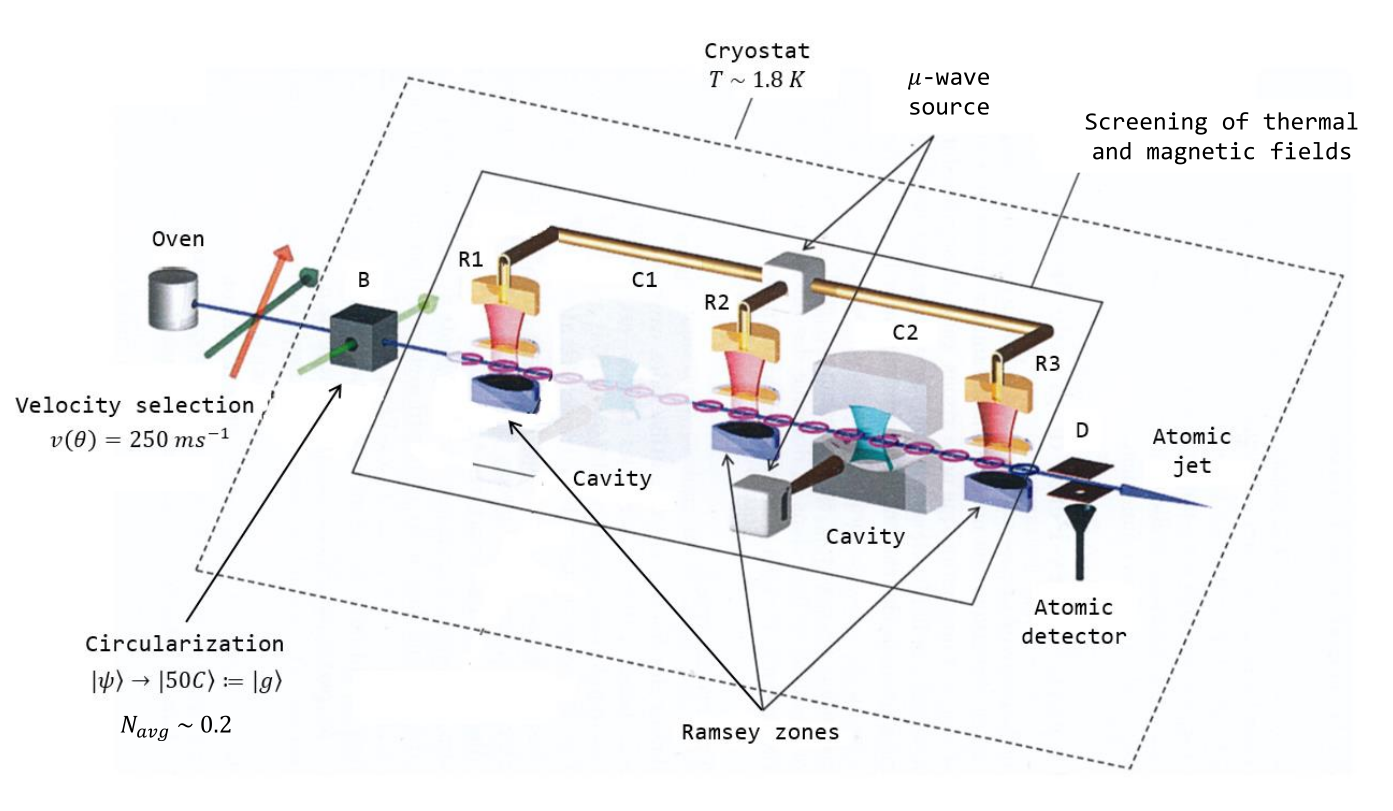
\includegraphics[width=\textwidth]{exp.png}
\end{frame}


\begin{frame}{Quantum information theory}

  \begin{block}{Shanon entropy}
    \[H(p_1,\ldots,p_n) = \sum_i -p_i\log (p_i)\]

  \vspace{-0.2cm}

  \end{block}

  \pause{}

  \begin{block}{VonNeuman Entropy}

  \vspace{-0.3cm}

    \[S(\rho) = -\Tr(\rho\log \rho) = H(p_1,\ldots,p_n) \gap \left(\rho = \sum p_i
      \ket {\psi_i}\bra{\psi_i}\right)\]

  \vspace{-0.2cm}

  \end{block}

  \pause{}

  \begin{block}{Mutual Infomation}
    \[I_{A:B} = S(\rho^A) + S(\rho^B) - S(\rho^{AB})\]
  \end{block}

  \pause{}

  \begin{block}{Reltative entropy to $\zeta$ (Kullback–Leibler divergence)}
    \[D(\rho) = \Tr(\rho (\log \rho - \log \zeta))\]
  \end{block}
\end{frame}

\begin{frame}{New second laws of thermodynamics}

  \[  \onslide<2->{- \Delta I_{QC:D} +}\Delta\beta Q \mathrel{\Alt<3>=\geqslant}
    \Alt<-2>0{\Delta D_{QC}}\]

\end{frame}

\begin{frame}{Second law}
  \centering
  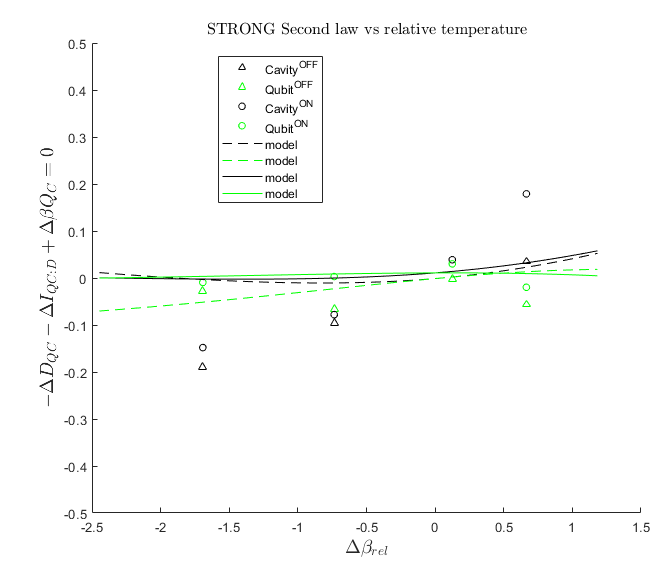
\includegraphics[height=\textheight]{plots/Strg1.png}
\end{frame}




\section{Deviation computation}

\begin{frame}{Monte-Carlo algorithm}

  \vspace{0.5mm}

  \begin{block}{Input}
    $n$ probabilities $p_i$ with standard deviation $\Delta p_i$
  \end{block}

  \pause{}
  \begin{block}{Goal}
    Simulate a corresponding probability distribution
  \end{block}

  \pause{}
  \begin{block}{Difficulty}
    We must project and truncate the distribution $\prod_i
    \mathcal{N}(p_i,\Delta p_i)$ to the polyhedron $\mathcal{P}$ of valid probability distributions
  \end{block}

  \pause{}
  \emph{Hit and run Markov chain}
  \begin{itemize}
  \item Take a random direction $d$
  \item Compute the segment $S = \{x_n + t d\} \cap \mathcal{P}$
  \item Project the distribution on that segment (it's a normal law)
  \item Draw $x_{n+1}$ from that distribution
  \end{itemize}

\end{frame}

\begin{frame}{Expectation and variance\onslide<4>{, Asymptotics}}
  \[I_h\onslide<4>{(N)} = \int_{\rho \in \mathcal{D}} h(\rho) e^{\onslide<4>{N}\ell(\rho)} P_0(\rho)\, \dd \rho.\]

  \pause{}

  \begin{block}{Expectation}

    \vspace{-1mm}

    \[\gap \gap \gap \gap E_h \onslide<4>{(N)}= \Alt<4>{\frac{I_h(N)}{I_1(N)}}{\frac{I_h}{I_1}} \gap \gap (I_1 = P(X=x))\]

    \vspace{-3mm}

  \end{block}

  \pause{}

  \begin{block}{Variance}

    \vspace{-3mm}

    \[\gap \gap V_h \onslide<4>{(N)}= E_{h_V} \onslide<4>{(N)}\gap h_v = \Alt<4>{{(h - \lim_{N \to \infty} E_h(N))}^2}{{(h - E_h)}^2}\]

    \vspace{-5mm}

  \end{block}


\end{frame}

\begin{frame}{Results in the interior}
  \begin{block}{Example of theorem}
    \[\int_{z \in U} g(z)e^{-\frac N2\|z\|^2} \dd z = g(0){\left(\frac
          {2\pi}{N}\right)}^{\frac n 2} +
      O\left({N^{-\frac n 2 -1}}\right)\]
  \end{block}

  \pause{}

  \emph{Example of proof}

  $g \in \class 1$ so $g(h) = g(0) + O(h)$, thus:
      \[\int g(z)e^{-\frac N2\|z\|^2} \dd z = \int
        g(0)e^{-\frac N2\|z\|^2} \dd z + \int O(h)e^{-\frac N2\|z\|^2} \dd z \]



\end{frame}

\newcommand{\lol}[1]{#1}

\begin{frame}{After multiples change of variables}

    \begin{block}{General case \onslide<3>{($g \in \class 1$)}}
  \[\int g(z)e^{N\ell(z)} \dd z = g(0) J_0+ O(e^{N\ell(0)} N^{-\frac n 2 -1})\]
\end{block}

  \vfill \pause{}

  \begin{block}{Case $g(0) = 0$ \onslide<3>{($g \in \class 3$)}}
    \[\int g(z)e^{N \ell(z)} \dd z =
      \tfrac{\Tr\left(-\partial^2 g(0) {\left(\partial^2 \ell(0)\right)}^{-1}\right)}{2N}
      J_0
      + O\left(e^{N\ell(0)}{N^{-\frac n 2 -2}}\right)\]
  \end{block}
\end{frame}

\begin{frame}{On the edge}
  \begin{block}{Example of edge theorem ($g \in \class1$)}

      \vspace{-4mm}

    \begin{multline*}
      \int x^m g(x,z)e^{-N(x + \frac 12 \|z\|^2)} \,\dd x\, \dd z =\\
      g(0,0)\,m! {(2\pi)}^{\frac n 2} N^{-\frac n 2 - m - 1} + O(N^{-\frac n 2 - m
        - 2})
    \end{multline*}

      \vspace{-3mm}

  \end{block}

  \pause{}

    \begin{block}{Other edge theorem ($g \in \class 2$, $g \in \class 3$ on $z$)}

      \vspace{-4mm}

    \begin{multline*}
      \int x^m g(x,z)e^{-N(x + \frac 12 \|z\|^2)} \,\dd x\, \dd z
    =\\ \frac{m!\Tr\left(\dparn g z 2\right)}{2N^{m+2}}
    {\left(\frac {2\pi}{N}\right)}^{\frac n 2}
    + O\left({N^{-\frac n 2 -m -3}}\right)
    \end{multline*}

      \vspace{-3mm}


  \end{block}



\end{frame}

\begin{frame}{After even more changes of variables}
  \[\Psi(x,\sigma,\zeta,\omega) = \exp\mat{0 &\omega\\-\omega^\dagger&0}
    \mat{x\sigma&0\\0&\Delta + \zeta - x \frac{I}r} \exp\mat{0 &-\omega\\\omega^\dagger&0}\]


  \begin{block}{General case \onslide<3>{($h \in \class 1$)}}
    \[I_h(N) = h(\rho\ml) I_1(N)+ O\left(\ldots\right)\]
  \end{block}

  \vfill \pause{}

  \begin{block}{Case $g(0) = 0$ \onslide<3>{($g \in \class 2$, but $g
        \in \class 3$ on $z =(\zeta,\omega)$)}}
    \[I_h(N) = \frac{\displaystyle \Tr \left( - \dparn h z 2 (\rho\ml)  \left( \dparn \ell z
            2(\rho\ml)\right)\inv\right)}{2N} I_1(N) + O(\ldots)\]
  \end{block}
\end{frame}

\begin{frame}{Final formulas}

  \begin{block}{Expectation ($h \in \class 1$)}
    \[E_A = h(\rho\ml) + O \left(\frac 1N\right)\]
  \end{block}

  \begin{block}{Variance ($h \in \class {\alert 1}$, and $h \in \class 3$ along
      the edge and inside)}

    If $\dparn h x 2 = o\left(\frac1x\right)$,

\vspace{-4mm}
    \[V_A = \Tr(\nabla h\pr \mathbb H\inv(\nabla h\pr)) + O \left(\frac 1{N^2}\right)\]

\vspace{-3mm}

    \begin{itemize}
    \item $A\pr$ is $A$ projected on tangent space to $\mathcal{D}$ in $\rho\ml$
    \item $\mathbb H$ is $\nabla^2f$ on the edge of $\mathcal{D}$ in
      $\rho\ml$
    \end{itemize}
  \end{block}
\end{frame}

\begin{frame}{Case of the entropy}


  \begin{block}{Expectation ($h \in \class \varepsilon$)}
    \[E_A = h(\rho\ml) + O \left(\frac 1{N^{\varepsilon}}\right)\]
  \end{block}

  \begin{block}{Variance ($h \in \class{\varepsilon}$, and $h \in \class 3$
      along the edge and inside)}
    If $\dpar h x = o\left(\frac 1 {x^\delta}\right)$, with $\delta < \varepsilon$,

\vspace{-4mm}

    \[V_A = \Tr(\nabla h\pr \mathbb H\inv(\nabla h\pr)) + O \left(\frac
        1{N^{1+\varepsilon - \delta}}\right)\]

\vspace{-3mm}

    \begin{itemize}
    \item $A\pr$ is $A$ projected on tangent space to $\mathcal{D}$ in $\rho\ml$
    \item $\mathbb H$ is $\nabla^2f$ on the edge of $\mathcal{D}$ in
      $\rho\ml$
    \end{itemize}
  \end{block}
\end{frame}




\section{Error propagation}

\begin{frame}{First order error propagation}
  \begin{center}
    Variance of $f(X)$?
  \end{center}
\[V(f(X)) \approx \nabla f^t V(X) \nabla f\]

\pause{}\vspace{5mm}

\begin{center}
By identification $\mathbb H^{-1}$ is the variance of $\rho\ml$
\end{center}

\end{frame}

\begin{frame}{Second law}
  \centering
  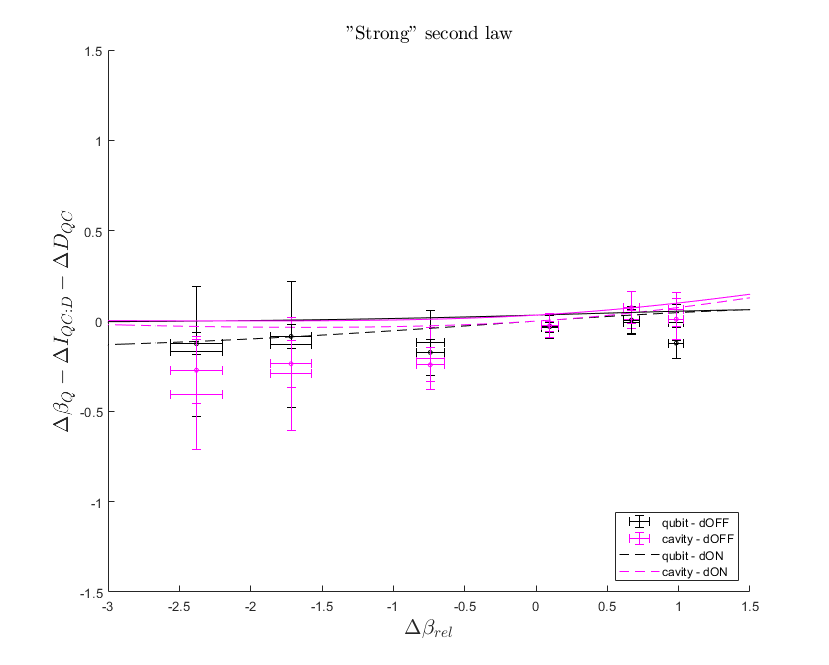
\includegraphics[height=\textheight]{plots/Strg2.png}
\end{frame}


\section{Centering the result}

\begin{frame}{The non-full span problem}

  \[\Span E_I \neq \mathcal{O}(\mathcal{H}) \implies \Alt<1>?{\dparn \ell \rho 2
    \not < 0}\]

  \onslide<3->

  \begin{center}
How to choose the \alert<3>{right} $\rho\ml$?
  \end{center}

  \onslide<4->

  \begin{center}
    There isn't a \alert<4>{right one}
  \end{center}


  \onslide<5->

  \begin{block}{Two objective optimization}
    Maximize a centering function $c$ among $\argmax_{\rho\in \mathcal{D}}\ell(\rho)$
  \end{block}

  \onslide<6->

  \begin{block}{How?}
  \onslide<7->
  Maximize $\ell + \varepsilon c$ then $\varepsilon \to 0$
  \end{block}


\end{frame}

\begin{frame}{Proposed centering function and properties}

  \begin{itemize}
  \item Log determinant ($\log \circ \det$)
  \item Von Neumann entropy ($S$)
  \end{itemize}

  \pause{}\vfill

  \begin{block}{Properties}
    \begin{itemize}
    \item Strictly concave
    \item Unitary invariant
    \item Give $\frac In$ as most centered matrix of $\mathcal{D}$
    \item Give exact result in dimension 2
    \end{itemize}
  \end{block}


\end{frame}

\begin{frame}{Log-determinant}
  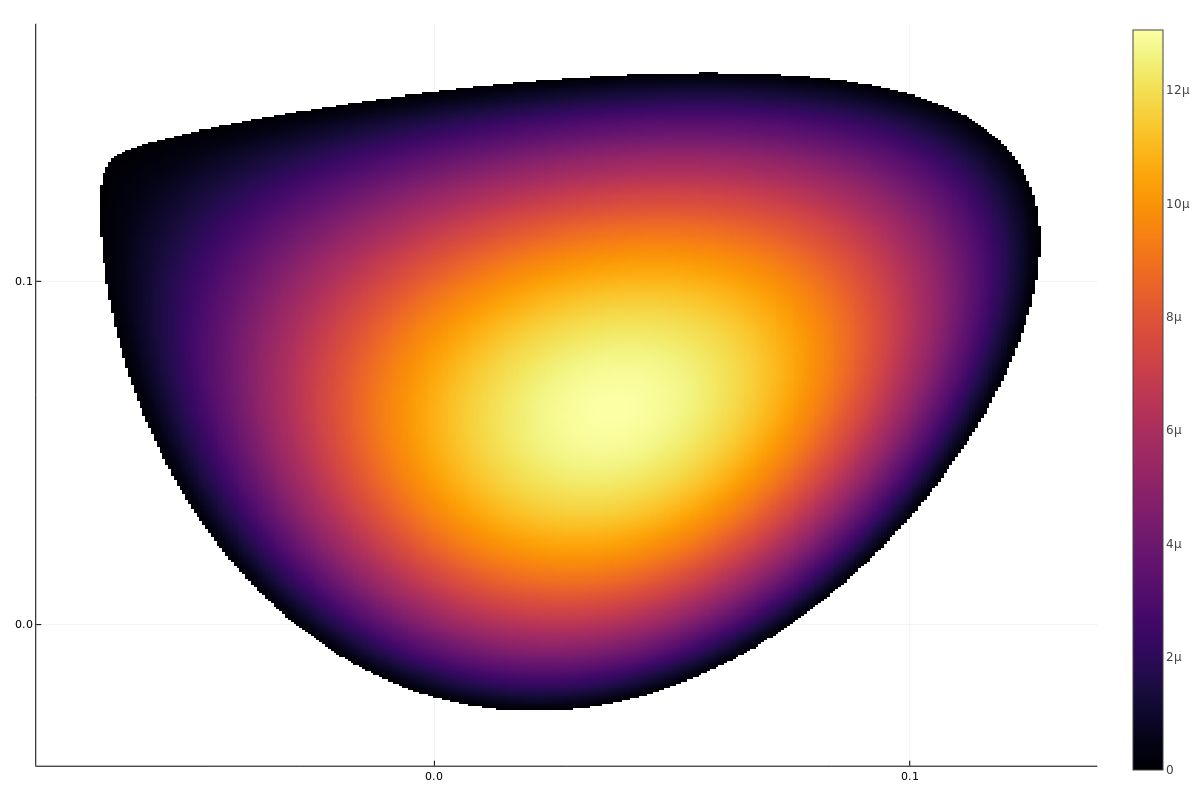
\includegraphics[width=\textwidth]{det5.png}
\end{frame}

\begin{frame}{Von-Neumann entropy}
  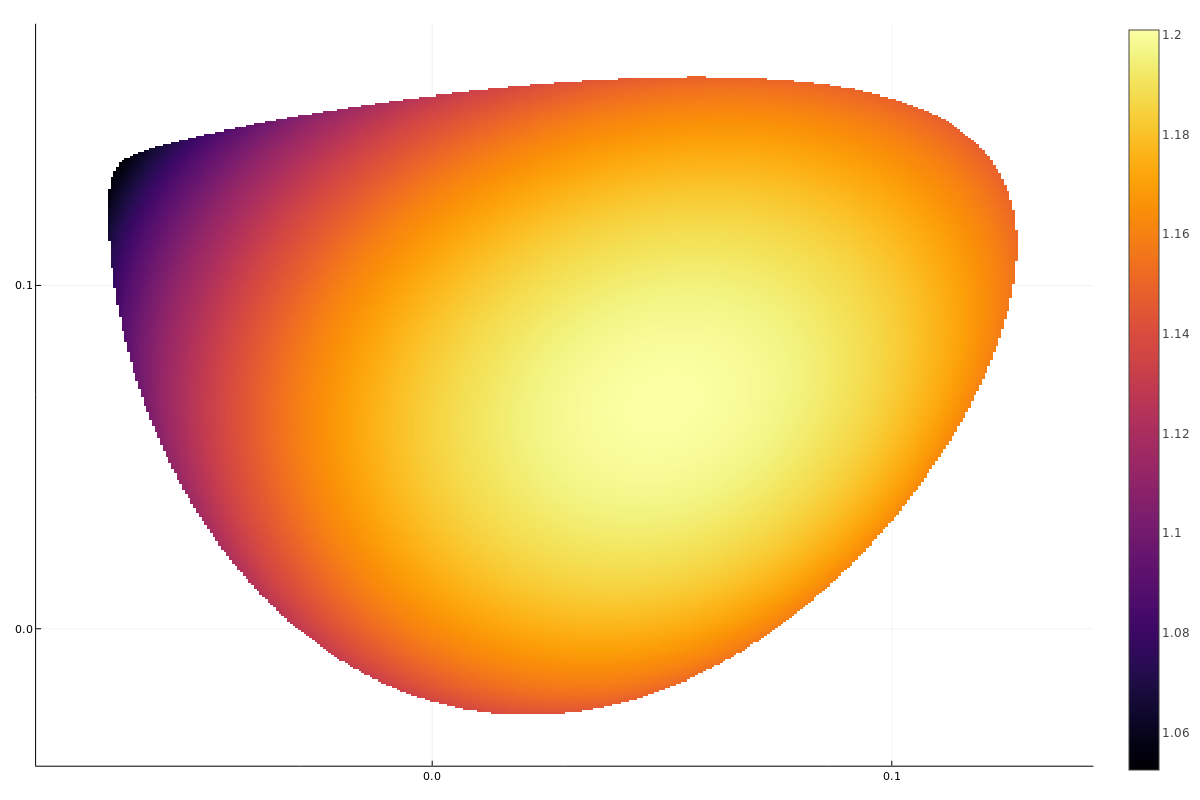
\includegraphics[width=\textwidth]{ent5.png}
\end{frame}




\section{Conclusion}

\begin{frame}{Conclusion}

  \begin{block}{Prior in Maths}
    \begin{itemize}
    \item Maxlike quantum state tomography
    \item Computed with projected gradient ascent
    \item Proof of convergence are asymptotic integrals development
    \end{itemize}
  \end{block}

  \pause{}

  \begin{block}{Prior in Physics}
    \begin{itemize}
    \item Quantum electro dynamics in cavities, Rabi oscillation
    \item Formalism of density matrices and quantum operations
    \item Quantum thermodynamics: information and entropy
    \end{itemize}
  \end{block}

  \pause{}

  \begin{block}{Personal Contribution}
    \begin{itemize}
    \item Monte-Carlo algorithm to evaluate error bars
    \item Extension of asymptotic proofs to allow entropy
    \item Creation of the secondary centering function system
    \end{itemize}
  \end{block}
\end{frame}

\begin{frame}{Thanks}

  \begin{itemize}
  \item Thanks to Igor Dotsenko for welcoming me in his lab and showing me
    their amazing experimental setup.
  \item Thanks to Pierre Rouchon for giving me interesting problems to solve and
    helping me solving them
  \item Thanks to Luis Najera for sharing with me his awesome internship project
    allowing me to directly apply my work to something physically interesting,
    and also for answering my various physical questions.
  \item Thanks to Valentin Metillon for helping me understanding various
    physical concepts.
  \end{itemize}

\end{frame}
\begin{frame}[standout]
  Thank you for your attention
\end{frame}






\end{document}

